\section{org::simtk::molecularstructure::Protein Class Reference}
\label{classorg_1_1simtk_1_1molecularstructure_1_1_protein}\index{org::simtk::molecularstructure::Protein@{org::simtk::molecularstructure::Protein}}
Inheritance diagram for org::simtk::molecularstructure::Protein::\begin{figure}[H]
\begin{center}
\leavevmode
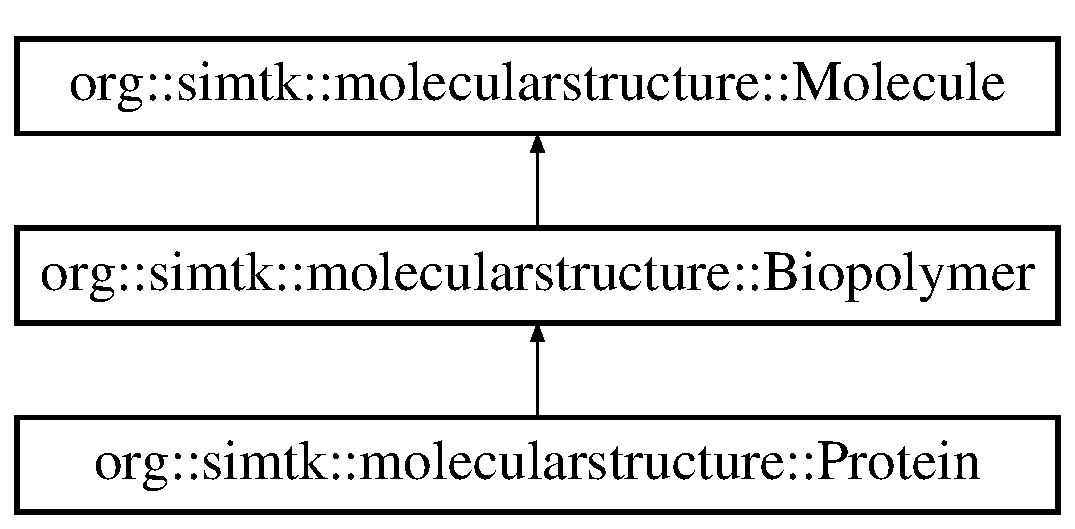
\includegraphics[height=3cm]{classorg_1_1simtk_1_1molecularstructure_1_1_protein}
\end{center}
\end{figure}


\subsection{Detailed Description}
\begin{Desc}
\item[Author:]Christopher Bruns\end{Desc}
TODO To change the template for this generated type comment go to Window - Preferences - Java - Code Style - Code Templates 



The documentation for this class was generated from the following file:\begin{CompactItemize}
\item 
C:/cygwin/home/cmbruns/eclipse/vtkjava/org/simtk/molecularstructure/Protein.java\end{CompactItemize}
